\documentclass[../Cours.tex]{subfiles}

\begin{document}
\chapitre{Horaires et durées}

\partie{Horaires}

\vocabulaire{Une année correspond à la durée d'un tour complet de la Terre autour du Soleil.}

\begin{center}
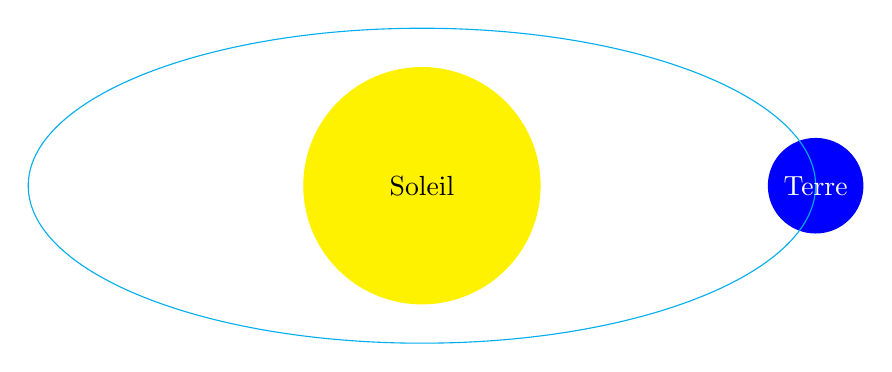
\begin{tikzpicture}
    \draw[yellow, fill=yellow] (0,0) circle (1.5);
    \node at (0,0) {Soleil};
    \draw[blue, fill=blue] (5,0) circle (0.6);
    \draw[cyan] (0,0) ellipse (5 and 2);
    \node[white] at (5,0) {Terre};
\end{tikzpicture}
\end{center}

\remarque{Année légale : 365 jours/366 jours\\Année tropique : 365,25 jours}

\vocabulaire{1 jour = 24 heures\\1 heure = 60 minutes\\1 minute = 60 secondes}

\remarque{1 jour = 8640 secondes\\1 heure = 3600 secondes}

\definition{Une horaire est un ou plusieurs nombres (en général représentant les heures et les minutes) permettant de décrire le temps écoulé depuis le début du jour (minuit).}

\begin{listedexemples}
    \item 11h42 $\longrightarrow$ onze heures et quarante-deux minutes
    \item 22h55 $\longrightarrow$ vingt-deux heures cinquante-cinq minutes
    \item $12:05$ pm $\longrightarrow$ midi cinq
\end{listedexemples}

\clearpage
\remarque{Format de l'heure anglaise
\begin{multicols}{4}
\begin{itemize}\small
    \item 00h $\rightarrow$ 12:00 am
    \item 01h $\rightarrow$ 01:00 am
    \item 02h $\rightarrow$ 02:00 am
    \item 03h $\rightarrow$ 03:00 am
    \item 04h $\rightarrow$ 04:00 am
    \item 05h $\rightarrow$ 05:00 am
    \item 06h $\rightarrow$ 06:00 am
    \item 07h $\rightarrow$ 07:00 am
    \item 08h $\rightarrow$ 08:00 am
    \item 09h $\rightarrow$ 09:00 am
    \item 10h $\rightarrow$ 10:00 am
    \item 11h $\rightarrow$ 11:00 am
    \item 12h $\rightarrow$ 12:00 pm
    \item 13h $\rightarrow$ 01:00 pm
    \item 14h $\rightarrow$ 02:00 pm
    \item 15h $\rightarrow$ 03:00 pm
    \item 16h $\rightarrow$ 04:00 pm
    \item 17h $\rightarrow$ 05:00 pm
    \item 18h $\rightarrow$ 06:00 pm
    \item 19h $\rightarrow$ 07:00 pm
    \item 20h $\rightarrow$ 08:00 pm
    \item 21h $\rightarrow$ 09:00 pm
    \item 22h $\rightarrow$ 10:00 pm
    \item 23h $\rightarrow$ 11:00 pm
\end{itemize}
\end{multicols}
}

\partie{Dates}

\convention{Forme simplifiée : Jour/Mois/Année\\
Forme développée : le [Nom du jour] Jour [Nom du mois] Année}

\exemple{Aujourd'hui :
\begin{itemize}
    \item Forme simplifiée : 19/01/2023
    \item Forme développée : le jeudi 19 janvier 2023
\end{itemize}}

\vocabulaire{\vspace{-3ex}
\begin{itemize}
    \item Un millénaire = 1000 ans
    \item Un siècle = 100 ans
    \item Une décennie = 10 ans
\end{itemize}
}

\paragraphe{rouge}{Norme}{ISO 8601}
\exemple{Le 2 mai 2022 à 13h57min12s en France : 2022-05-02T13:57:12+02:00\\
\begin{center}
\begin{tikzpicture}
    \node at (0,0) {2022~-~05~-~02~T~13~:~57~:~12~+~02~:~00};
    \node[rouge] at (-3.6,-0.5) {année};
    \node[rouge] at (-2.3,-0.5) {mois};
    \node[rouge] at (-1.2,-0.55) {jour};
    \node[rouge] at (0,-1) {heures}; \draw[Latex-,rouge] (-0.2,-0.25) -- (-0.2,-0.8);
    \node[rouge] at (0.8,-0.5) {minutes};
    \node[rouge] at (1.8,-1) {secondes}; \draw[Latex-,rouge] (1.8,-0.25) -- (1.8,-0.8);
    \node[vert] at (4,-0.5) {fuseau horaire}; \draw[vert] (2.1,-0.3) rectangle (4.3,0.3);
\end{tikzpicture}
\end{center}
}

\clearpage
\partie{Conversion}
\exemple{Convertir \qty{1245}{\second} en minutes et secondes}
\methode{On effectue une division euclidienne.}

\begin{center}
    \begin{tikzpicture}
        \node at (0,0) {\opidiv[displayintermediary=all,dividendbridge]{1245}{60}};
        \draw[vert] (-0.4,-1.6) rectangle (0.5,-1.05);
        \draw[rouge] (0.9,0.5) rectangle (1.7,0.95);
        \node[anchor=west] at (3,0) {\qty{1245}{\second} $=$ 20 minutes et 45 secondes};
        \draw[rouge] (5.3,-0.25) -- (5.8,-0.25);
        \draw[vert] (8.4,-0.25) -- (9,-0.25);
    \end{tikzpicture}
\end{center}

\exemple{Convertir \qty{7345}{\second} en heures, minutes et secondes}
\methode{On va effectuer deux divisions euclidiennes.}

\begin{center}
    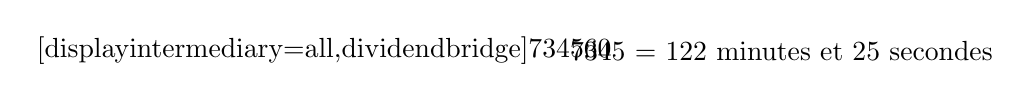
\begin{tikzpicture}
        \node at (0,0) {\opidiv[displayintermediary=all,dividendbridge]{7345}{60}};
        \node[anchor=west] at (3,0) {\qty{7345}{\second} $=$ 122 minutes et 25 secondes};
    \end{tikzpicture}
\end{center}
\begin{center}
    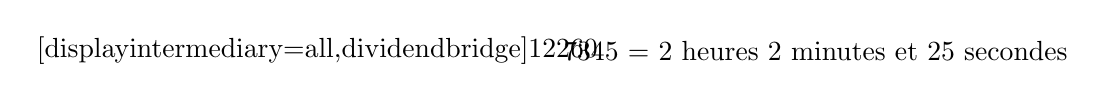
\begin{tikzpicture}
        \node at (0,0) {\opidiv[displayintermediary=all,dividendbridge]{122}{60}};
        \node[anchor=west] at (3,0) {\qty{7345}{\second} $=$ 2 heures 2 minutes et 25 secondes};
    \end{tikzpicture}
\end{center}

\exemple{Combien y a-t-il de secondes dans 5h25min13s ?}
\methode{On va multiplier les heures par 3600, et les minutes par 60.}

\begin{align*}
    \mbox{5h25min13s} &= 5 \times 3600 + 25 \times 60 + 13 \\
    &= 18000 + 1500 + 13\\
    &= \qty{19513}{\second}
\end{align*}

\clearpage
\EXERCICES 
\begin{questions}
    \exercicetitre{Addition de durées}
    \question 2h35 + 4h43 = 
    \question 6h28 + 9h12 = 
    \question 8h37 + 9h12 = 
    
    \exercicetitre{Calculer les durées}
    \question Si un film commence à 17h29 et dure 2 heures et 15 minutes, à quelle heure se termine-t-il ?
    \question Si une personne part de chez elle à 6h14 et met 1 heure et 32 minutes pour arriver au travail, à quelle heure arrive-t-elle ?
    \question Si un train part à 12h52 et met 5 heures et 12 minutes pour arriver à destination, à quelle heure arrive-t-il ?
    
    \exercicetitre{Comparaison d'horaires}
    \question Si un train part à 7h14 et met 2 heures et 45 minutes pour arriver à destination, à quelle heure arrivera un train qui part à 8h29 ?
    \question Si un avion décolle à 11h52 et met 8 heures et 18 minutes pour arriver à destination, à quelle heure arrivera un avion qui décolle à 13h10 ?
    \question Si un match de football commence à 19h29 et dure 2 heures et 45 minutes, à quelle heure se termine un match qui commence à 20h44 ?

    \exercicetitre{Dates}
    \question Si le 13 mars tombe un vendredi, quel jour est-il le 1er avril ?
    \question Cette année Pâques tombe le 9 avril 2023. Quel jour sera le jeudi de l'Ascension ?
    \question Le 1er janvier 2023 est un dimanche. Quel jour sera le 1er janvier 2024 ?

    \exercicetitre{Convertir en hh:mm:ss}
    \question \qty{81702}{\second}
    \question \qty{17384}{\second}
    \question \qty{86400}{\second}

    \exercicetitre{Combien y a-t-il de secondes dans :}
    \question 3h52min41s
    \question 12h00min06s
    \question 22h05min17s

    
\end{questions}

\end{document}